\chapter{Kernel contraction}
\label{kernel}
Belief contraction is the process of removing beliefs from belief bases. In Chapter \ref{background}, we discussed the difference between belief bases and belief sets. In this study, we perform kernel contraction on belief bases. It can be done by either of two ways. The first way is selecting subsets of the belief base that do not logically imply the belief to be removed. This is called the \textit{remainder set} approach. It works by finding the largest subsets of the belief base, such that those subsets do not imply the removed belief. For example, the knowledge base:
\begin{center}
$\lbrace a, a \rightarrow b, b, c \rbrace$
\end{center}
has two remainder sets that do not logically imply $b$:
\begin{center}
$\lbrace a, c\rbrace, \lbrace a \rightarrow b, c\rbrace$
\end{center}
And they are the largest such subsets. This means that there are no larger subset of the original set that do not imply $b$. So we can choose one of them (or, in the general case, the intersection of more than one\footnote{This is called \textit{partial meet contraction.}}) to be the new (contracted) belief base.


The other approach is done by incising all the minimal subsets that logically imply the removed belief; by ``incising'' we mean removing a member from the set. This second approach is the one we are going to focus on in this study. If a set $K$ of beliefs imply a belief $\alpha$, and $K$ is the minimal such set (no proper subset of $K$ implies $\alpha$), removing one element of $K$ will guarantee that it does not imply $\alpha$. Contraction is done here by finding all such minimum subsets and removing an element from each of them. We call such minimal sets \textit{kernels}. Kernels will be discussed in more details in the coming section. But we need to go over some example first.

Consider the same set:
\begin{center}
$ \lbrace a, a \rightarrow b, b, c \rbrace $
\end{center}
To contract the set by $b$, it is not enough to remove $b$ from the set. If we do so, we get:
\begin{center}
$ \lbrace a, a \rightarrow b, c \rbrace $
\end{center}
which still implies $b$. We need to prevent the resulting set of beliefs from implying $b$. The minimal subset that implies $b$ is 
\begin{center}
$ \lbrace a, a \rightarrow b \rbrace $
\end{center}
We call it a $b$-kernel. Since the kernel is a minimal subset that implies $b$, removing only one element of that kernel is enough to make it not imply $b$. The only other $b$-kernel of the original set is $\lbrace b \rbrace$; we can only break this kernel by removing $b$. Breaking the other kernel can be done either by removing $a$, or by removing $a \rightarrow b$. So the two possible resulting belief bases after contraction are:
\begin{center}
$ \lbrace a, c \rbrace $ and $ \lbrace a \rightarrow b, c \rbrace $
\end{center}
This is how kernel contraction works. Every $b$-kernel is one way to infer $b$. To contract $b$ every kernel should be broken by removing at least one belief. 

Kernel contraction can be composed of two main steps: computing kernels, and cutting them. In this chapter, we will discuss kernels and see how they can be defined formally. We will discuss briefly how to compute kernels using an algorithm called \textit{pinpointing}. Assuming we have a set of kernels that we computed, we will discuss previous work done on cutting kernels that will give us a good basis for introducing the new approaches afterwards. Then we will discuss the hitting-set approach to contraction in the context of \textit{minimal change} requirement. Last topic to be discussed in this chapter will be our new graph approach kernel contraction. The algorithm will combine the two steps of kernel contraction (computing and cutting). It will be followed by some analysis and comparisons between different examples using it.


\section{What are kernels?}
Kernel contraction was introduced by Hansson\cite{kernel} as a variant of an older approach called ``safe contraction''\cite{safe}. In both approaches, contracting a knowledge base \textbf{K} by $\alpha$ is done by discarding beliefs that contribute to make \textbf{K} imply $\alpha$. Beliefs that contribute to make \textbf{K} imply $\alpha$ are members of some $\alpha$-kernels of \textbf{K}, and all members of every $\alpha$-kernel contribute to make \textbf{K} imply $\alpha$. In the previous example, there were two $b$-kernels: $\lbrace b \rbrace$ and $\lbrace a, a \rightarrow b \rbrace$. We need to remove at least one element from each kernel to contract the original set by $b$. We refer to the set of $\alpha$-kernels of \textbf{K} by $\textbf{K} \perp \alpha$.
\begin{defn}(Kernel Set)
According to \cite{hansson}, for a belief base \textbf{K} and a belief $\alpha$, $\textbf{K} \perp \alpha$ is a set such that $X \in \textbf{K} \perp \alpha$ if and only if:
\begin{enumerate}
\item $X \subseteq \textbf{K}$,
\item $X \vdash \alpha$, and
\item if $Y \subset X$ then $Y \nvdash \alpha$.
\end{enumerate}
$\textbf{K} \perp \alpha$ is a kernel set that contains all $\alpha$-kernels of \textbf{K}.
\end{defn}
Kernels are the smallest subsets of the knowledge base that imply a specific belief. Therefore, in order to give up that belief, every one of those kernels needs to be incised. If those kernels are not ``minimal'', they might contain some beliefs that do not contribute to make the kernel imply that specific belief. For example, in $\lbrace \alpha, \beta \rbrace$, $\beta$ is a belief that does not contribute to make the set imply $\alpha$. In that case, removing $\beta$ only would not help in giving up $\alpha$. 

So, because of the minimality of the kernels, every belief in the kernel is significant to implying the belief that we want to give up ($\alpha$). And that's why removing one belief from a kernel is sufficient to make that kernel not imply $\alpha$. So, we use a function that cuts every kernel in the kernel set. We call such function an \textit{incision function}; it takes a set of kernels and removes an element from each kernel. 

The incision function is defined in \cite{hansson} as follows:
\begin{defn}(Incision function)
An incision function $\sigma$ is a function such that for all beliefs $\alpha$:
\begin{enumerate}
\item $\sigma (A \perp \alpha) \subseteq \bigcup (A \perp \alpha)$
\item If $\phi \neq X \in A \perp \alpha$, then $X \cap \sigma (A \perp \alpha) \neq \phi$
\end{enumerate}
\end{defn}
Contraction is done by removing the beliefs that are selected by the incision function from the original knowledge base. Contraction $\approx_\sigma$ using the incision function $\sigma$ can be defined as:
\begin{defn}\cite{hansson} (Contraction)
\begin{center}
$A \approx_\sigma \alpha = A \smallsetminus \sigma (A \perp \alpha)$
\end{center}
\end{defn}


\section{Computing kernels}
Kernel contraction is about contracting knowledge bases using kernels. Kernels are the minimal subsets of the knowledge base that imply a certain consequence. The incision function can perform the contraction by cutting through all kernels of a specific belief. So, the first step in contraction is computing all kernels that imply the belief that needs to be removed. For that purpose, we use the pinpointing algorithm introduced in \cite{pin}.

To show how the algorithm works, we use the example introduced in \cite{pin}. Given an $\mathcal{EL}$ $TBox$ $\mathcal{T}$ consisting of the following four GCI axioms:
\begin{center}
$\mathcal{T} = \lbrace ax_1: A \sqsubseteq \exists{r}.A$, \hspace{7pt}  $ax_2: A \sqsubseteq Y$,  \hspace{7pt} $ax_3: \exists{r}.Y \sqsubseteq B$, \hspace{7pt} $ax_4: Y \sqsubseteq B \rbrace$,
\end{center}
we can see that $A \sqsubseteq B$ holds according to $\mathcal{T}$, i.e. $A \sqsubseteq_{\mathcal{T}} B$. Let: 
\begin{center} 
$\alpha = A \sqsubseteq B$.
\end{center}
According to the definition of kernel sets:
\begin{center}
$\mathcal{T} \perp \alpha = \lbrace \lbrace ax_2, ax_4 \rbrace, \lbrace ax_1, ax_2, ax_3 \rbrace \rbrace$
\end{center}
The algorithm introduced in \cite{pin} computes all kernels using a modified version of the $\mathcal{EL}$ subsumption algorithm. It works by finding a monotone boolean formula called \textit{``pinpointing formula''}. The propositions of the pinpointing formula are GCIs of the $TBox$, and a propositional \textit{valuation} represents the kernels. In that sense, a valuation is a set of propositional variables that satisfy the formula, and these variables are the GCIs that constitute a kernel. So, by finding all valuations of the pinpointing formula we can get all kernels.

In the worst case, this approach takes exponential time (w.r.t the size of the $TBox$) to find all kernels. This is the case when there are exponentially many kernels. However, \cite{pin} also gives a polynomial-time algorithm that computes only one kernel. Because it is not part of the scope of this study, we are not going to discuss and analyze details of the pinpointing algorithm. All that matters is the worst-case time complexity, as it will affect the complexity of the kernel contraction algorithm that uses it.


\section{Previous work}
We now know we can use the pinpointing algorithm to get the set of all kernels. We then need to remove one element from each kernel to perform contraction. This is the role of the incision function; it picks an element from each kernel so that it cuts through all kernels.
In this section, we look at some of the incision function implementations discussed in \cite{zwei}. The goal of this study is to continue the work started in \cite{zwei}, and to revise some of what has already been done. 

Given an $\mathcal{EL}$ $TBox$ $\mathcal{T}$ and a belief $\alpha$, ($\mathcal{T} \perp \alpha$) is the set of $\alpha$-kernels. The main contraction algorithm is shown in Algorithm \ref{MainAlgorithm}.

\begin{algorithm}
\caption{Contraction algorithm}
\label{MainAlgorithm}
\begin{algorithmic}[1]
\Procedure{contract}{$ \mathcal{T} $, A}
\State kernelset = \Call{pinpoint}{$ \mathcal{T} $, A}
\State giveUpSet = \Call{cut}{kernelset}
\State $\mathcal{T}$ = $\mathcal{T}$ / giveUpSet
\EndProcedure
\end{algorithmic}
\end{algorithm}

``kernelset'' refers to ($\mathcal{T} \perp \alpha$), and \textit{giveUpSet} is the set of beliefs selected by the incision function (CUT) to be removed. The algorithm is straightforward. It works by generating the set of kernels using the pinpoint formula as discussed in the previous section. Then it calls the incision function that picks up beliefs from every kernel, ensuring that it cuts all kernels. The beliefs are then removed from the knowledge base, i.e. from the $TBox$.

This general approach can be used with different incision functions. The call to the CUT function can be replaced with a call to another implementation of the incision function. The first implementation is the most straightforward one, where it removes a random belief from every kernel. This is given in Algorithm \ref{RandomAlgorithm}.

\begin{algorithm}
\caption{Random removal}
\label{RandomAlgorithm}
\begin{algorithmic}[1]
\Function{RandomRemove}{kernelset}
\State giveUpSet = $\lbrace \rbrace$
\For{$kernel \in kernelset$} 
\State choose a random belief $\alpha$ from $kernel$
\State giveUpSet = giveUpSet $\cup$ $\lbrace \alpha \rbrace$
\EndFor \State
\Return giveUpSet
\EndFunction
\end{algorithmic}
\end{algorithm}

The time complexity of RandomRemove function is polynomial: $O(m)$, where $m$ is the number of kernels (size of the kernelset), assuming that the random selection takes constant time. However, this is clearly not a good algorithm. In this example:
\begin{center}
kernelset = $\lbrace \lbrace a, c \rbrace, \lbrace b, c \rbrace \rbrace$, 
\end{center}
one of the possible outcomes of the RandomRemove algorithm is:
\begin{center}
\textit{giveUpSet} = $\lbrace c, b \rbrace$
\end{center}
which unnecessarily removes $b$. This could happen when the algorithm selects $c$ from the first kernel and $b$ from the second kernel. This solution:
\begin{center}
\textit{giveUpSet} = $\lbrace c \rbrace$
\end{center}
seems more concise and removes less beliefs. The second solution could be obtained if the algorithm is smart enough to check if the second kernel has already been incised. 

The next algorithm (Algorithm \ref{RandomExclusionAlgorithm}) does this. It goes over all kernels, and randomly selects a formula from every kernel to be removed. Every time it selects a belief, it marks all kernels that contain that belief so that they are not considered for belief removal in the following iterations. 

\begin{algorithm}
\caption{Random removal with exclusion}
\label{RandomExclusionAlgorithm}
\begin{algorithmic}[1]
\Function{RandomRemoveAndExclude}{kernelset}
\State giveUpSet = $\lbrace \rbrace$
\For{i=0 to size(kernelset)-1} 
\State kernelset[i].valid = true
\EndFor \State
\For{i=0 to size(kernelset)-1}
\If{kernelset[i].valid == true}
\State choose a random belief $\alpha$ from kernelset[i]
\State giveUpSet = giveUpSet $\cup$ $\lbrace \alpha \rbrace$
\For{j=i to size(kernelset)-1}
\If{kernelset[j].contains($\alpha$)}
\State kernelset[j].valid = false
\EndIf
\EndFor
\EndIf
\EndFor \State
\Return giveUpSet
\EndFunction
\end{algorithmic}
\end{algorithm}

Algorithm \ref{RandomExclusionAlgorithm} has a worst-case time complexity of $O(n^2)$, where $n$ is the size of the kernel set, assuming that kernels are stored as hash tables so ``kernelset[j].contains($\alpha$)'' takes constant time. If the kernels are stored as ordered lists, the time complexity would increase to become $O(n^2 \cdot \ln m)$, where $m$ is the size of the largest kernel. If kernels are unordered lists, the time complexity is $O(n^2 \cdot m)$. The second main loop has another nested loop inside it, and neither of them takes more than $n$ steps to finish. 

\subsection{Greedy Contraction}
The greedy approach works by selecting the beliefs that appear in more kernels to be removed before those that appear in less kernels. At each step, the algorithm finds which belief appears the most in kernels and removes it, and then it forgets about those kernels (it does not consider those kernels that contain the removed belief for the following steps). This means that if a belief is selected for removal, all the kernels that contain it are already incised and no more beliefs need to be removed from these kernels.

\begin{algorithm}
\caption{Greedy Selection}
\label{GreedyAlgorithm}
\begin{algorithmic}[1]
\Function {GreedyContract}{$kernelset, beliefs$}
\State $initializeValidKernels(kernelset)$
\State $initializeBeliefOccurrences(beliefs)$ 
\State $computeOccurrences(kernelset, beliefs)$ 
\State \Return $selectMaxBeliefs($kernelset, beliefs$)$
\EndFunction
\end{algorithmic}
\end{algorithm}

\begin{algorithm}
\begin{algorithmic}[1]
\State // Mark all kernels as not cut to keep track of the remaining kernels to be cut
\Function{initializeValidKernels}{$kernelset$}
\State $validKernels = 0$ $// global \: variable$
\For{$i = 1$ to $size(kernelset)$}
\State $validKernel[i] = 1$  $// global \: array$
\State $validKernels = validKernels + 1$
\EndFor
\EndFunction
\end{algorithmic}

\begin{algorithmic}[1]
\State // Create an array to count the number of kernels that include each belief
\Function{initializeBeliefOccurrences}{$beliefs$}
\For{$i = 1$ to $size(beliefs)$}
\State $occurs[i] = 0$  $// global \: array$
\EndFor
\EndFunction
\end{algorithmic}
\end{algorithm}

\begin{algorithm}
\begin{algorithmic}[1]
\State // For each belief, compute the number of kernels that include it
\Function{computeOccurrences}{$kernelset, beliefs$}
\For{$i=1$ to $size(beliefs)$}
\For{$j=1$ to $size(kernelset)$}
\If{$kernelset[j].contains(beliefs[i])$}
\State $occurs[i] = occurs[i] + 1$
\EndIf
\EndFor
\EndFor
\EndFunction
\end{algorithmic}
\end{algorithm}

\begin{algorithm}
\begin{algorithmic}[1]
\State // Select the belief that appears in biggest number of kernels, and add to giveUpSet
\Function{selectMaxBeliefs}{$kernelset, beliefs$}
\State $giveUpSet = \lbrace \rbrace$
\While{$validKernels > 0$}
\State $max = 0$
\State $maxIndex = 0$

\State // search for the belief with max number of occurrences
\For{$i=1$ to $size(beliefs)$}
\If{$occurs[i]>max$}
\State $max = occurs[i]$
\State $maxIndex = i$
\EndIf
\EndFor

\State // add the selected belief from the containing kernels to giveUpSet and update count
\For{$i=1$ to $size(kernelset)$}
\If{$kernelset[i].contains(beliefs[maxIndex])$}
\State $validKernel[i] = 0$
\State $validKernels = validKernels - 1$
\State updateOccurrences($kernelset[i], beliefs$)
\EndIf
\EndFor
\State $occurs[maxIndex] = 0$
\State $giveUpSet = giveUpSet \cup \lbrace beliefs[maxIndex] \rbrace$
\EndWhile
\State \Return $giveUpSet$
\EndFunction
\end{algorithmic}
\end{algorithm}

\begin{algorithm}
\begin{algorithmic}[1]
\State // disregard the given kernel from the kernels that include each belief
\Function{updateOccurrences}{$kernel, beliefs$}
\For{$i=1$ to $size(kernel)$}
\State $removeOccurances(beliefs, kernel[i])$
\EndFor
\EndFunction
\end{algorithmic}

\begin{algorithmic}[1]
\State // decrement the number of kernels that include the given belief
\Function{removeOccurrences}{$beliefs, belief$}
\For{$i=1$ to $size(beliefs)$}
\If{$beliefs[i] == belief$}
\State $occurs[i] = occurs[i] - 1$
\EndIf
\EndFor
\EndFunction
\end{algorithmic}
\end{algorithm}

Algorithm \ref{GreedyAlgorithm} explains how the greedy approach for contraction works. Given a set of kernels and the set of all beliefs (the knowledge base), it proceeds as follows: it computes the number of occurrences of every belief in the kernels given, then it removes them one by one starting from the beliefs with maximum number of occurrences, until all kernels are incised. It does not actually remove the beliefs, but it collects them in the $giveUpSet$ that will be returned to the main contraction, which in turn will remove them from the knowledge base. So the greedy approach can be embedded in the main algorithm as a way to choosing the beliefs that need to be removed. 
	
The worst-case time complexity of the greedy algorithm is lower-bounded by the complexity of the ``while'' loop in the $selectMaxBeliefs()$ function. If the size of $beliefs$ is $m$, the size of $kernelset$ is $n$, and the size of the biggest $kernel$ is $k$, then the worst-case time complexity is $O(n^2 \cdot k \cdot m)$. This could be significantly enhanced by using more clever data structures to make the invalidation of the kernels (the step where we decrement the number of valid kernels and update the occurrences) faster.


\section{Minimal change}
According to the information economy principal (minimality), in every change of the epistemic state, loss of information should be minimum\cite{econ}. This means that a system should choose an epistemic change outcome that minimizes loss of information. To satisfy the requirement of the minimum change we need an algorithm that removes the least number of GCIs while hitting all the kernels; but the kernels are nothing but sets of beliefs (GCIs). Luckily, this is exactly the \textit{minimal hitting set problem}, which already has some relatively efficient algorithms that we can use here. 

\subsection{Hitting set approach}
Another (more efficient) approach to cutting kernels to perform contraction is the hitting set algorithm. The minimal hitting set problem is defined as follows:
\begin{defn}\cite{hit}
Given a set $S=\{s_{1}, s_{2}, ..., s_{n}\}$ of $n$ non-empty sets, a minimal hitting set $d$ is a set such that:
\begin{center}
$\forall_{s_{i} \in S} [ s_{i} \cap d \neq \emptyset] \wedge \nexists_{d' \subset d}[\forall_{s_{i} \in S} (s_{i} \cap d' \neq \emptyset) ]$
\end{center}
\end{defn}

Thus, $d$ is a minimal hitting set if and only if it contains at least an element from every set, and no proper subset of it is a hitting set. In the context of kernel contraction in $\mathcal{EL}$, we can define the minimal hitting set contraction as:
\begin{defn}(Minimal hitting set contraction)
Given a kernelset $K=\{k_{1}, k_{2}, ..., k_{n}\}$ of $n$ kernels, a minimal hitting set $giveUpSet \subset K$ is a set such that:
\begin{center}
$\forall_{k_{i} \in K} [ k_{i} \cap giveUpSet \neq \emptyset] \wedge \nexists_{giveUpSet' \subset giveUpSet}[\forall_{k_{i} \in K} (k_{i} \cap giveUpSet' \neq \emptyset) ]$
\end{center}
\end{defn}

Since kernels are subsets of the $TBox$, and our goal to find a $giveUpSet$ that hits all kernels, we can use approaches to the minimal hitting set problem to solve it. There are good approximation algorithms, such as the one introduced in \cite{hit}, for the minimal hitting set problem, that are feasible in terms of running time. 

The notion of \textit{minimality} can be interpreted in terms of set-containment or cardinality. We call a hitting set minimal in terms of caridnality if there is no smaller-sized set that is a hitting set. However, the interpretation we use here is minimality accoring to set-containment; this means a minimal hitting set is a hitting set that has no proper subset that is a hitting set. So there might exist different minimal hitting sets with different cardinalities, but none of them is subsumed by a proper subset that is a hitting set\cite{hit}. But our goal was to satisfy the information economy principal by removing hitting sets with minimum cardinality. 

For that reason, after getting all minimum hitting sets, we need to consider only the ones that are smallest in size. For the kernel set:
\begin{center}
$kernelset = \lbrace \lbrace a, b \rbrace , \lbrace a, c \rbrace \rbrace$,
\end{center}
there are two minimal hitting sets:
\begin{center}
$\lbrace a \rbrace$ \hspace{1cm} and \hspace{1cm} $\lbrace b, c \rbrace$
\end{center}
and they are of different sizes. The following step then is to determine that the smallest of them should be selected for contraction, which is $\lbrace a \rbrace$.

We can now use one of the minimal hitting set algorithms combined with the cardinality selection step to implement contraction for a $TBox$, by implementing the minimal incision function that adopts them, to achieve minimum change (which we can call then, a \textit{minimal incision function}). We are not going to implement such a function in this study, but for now, we will assume that there is a function:
\begin{verbatim}
 min-hit-CUT(kernelSet)
\end{verbatim}
that takes a set of kernels, and returns a minimal hitting set (minimal in both set-containment and cardinality) of sentences to give up. We can use this function, as if it is implemented, and may implement it in some future work.

\subsection{Graph approach}
Now, we introduce another technique for kernel contraction in $\mathcal{EL}$ that is based on graphs. The reason why following graph approach is useful in solving contraction problem is that we are performing contraction of $TBoxes$, and they have an implicit graph-like hierarchy. 

An $\mathcal{EL}$ $Tbox$ consists of GCIs (we can transform all definition formulas to GCIs), that can be seen as nodes and edges. A GCI can be thought of as a directed edge between two nodes representing concepts on the two sides of the subsumption symbol ($\sqsubseteq$). So reasoning with $TBoxes$ is similar to reasoning with directed graphs. We can reduce $TBox$ reasoning problems to graph problems and use graph algorithms to solve them. The subsumption relationship that forms a $TBox$ seem to have an intuitive interpretation as a directed graph; and that's why we might use the word ``subsumption hierarchy'' later in this study to denote the relationship between concepts in the $TBox$.

The $\mathcal{EL}$ subsumption algorithm described in \cite{small} uses a graph approach, perhaps because it is intuitive to think of $TBoxes$ as graphs. A lot of work has been done in the area of Graph Theory, which makes it easy to use the already existing algorithms to solve some graph problems. Also, graphs are easy to imagine and work with. 

Our goal is to reduce the kernel contraction problem to a graph problem, and, using some efficient graph algorithms to perform kernel contraction. The algorithm we build here starts by transforming the $TBox$ into a graph. Then, it generates all kernels by finding all paths that imply the formula we are contracting. After that, it removes one formula from each kernel by removing an edge from each path, since paths here represent kernels (this will all be explained shortly). Finally it transforms the graph back into a $TBox$. 

We will start by describing the algorithm in details, and then explain each of its main steps. 

\subsubsection{Main algorithm}
%Every GCI of the form $C \sqsubseteq D \sqcap E$ can be decomposed into two GCIs: $C \sqsubseteq D$ and $C \sqsubseteq E$, where $C$, $D$ and $E$ are arbitrary concept expressions. 
Given an $\mathcal{EL}$ $TBox$ $\mathcal{T}$, and a GCI $\mathbb{A}$ (where $\mathbb{A}$ is in the form of $C \sqsubseteq D$, such that $C$ and $D$ are arbitrary concept expressions), we contract $\mathcal{T}$ by $A$ using Algorithm \ref{GraphContract}:


\begin{algorithm}
\caption{Contraction using graph approach}
\label{GraphContract}
\begin{algorithmic}[1]
\Function {graphContract}{$ \mathcal{T} $, $\mathbb{A}$}
\State complete($ \mathcal{T} $)
\State G = transform($ \mathcal{T} $)
\State C = $arg_{left}(\mathbb{A})$ $//$ gets the concept expression on the left side of the GCI
\State D = $arg_{right}(\mathbb{A})$ $//$ gets the right-side concept expression
\State paths = getPaths(G, C, D)
\State cutPaths(G, paths)
\State $ \mathcal{T} $ = de-transform(G)
\EndFunction
\end{algorithmic}
\end{algorithm}

The complete function in step 2 uses the $\mathcal{EL}$ subsumption algorithm to compute all subsumptions of $\mathcal{T}$. All the subsumptions computed are added to $\mathcal{T}$. The subsumption algorithm proceeds in four steps:\cite{new}
\begin{enumerate}
\item Normalize the $TBox$.
\item Translate the normalized $TBox$ into a graph.
\item Complete the graph using completion rules.
\item Read off the subsumption relationship from the normalized graph.
\end{enumerate}
The algorithm is explained in full details in \cite{new}. We now need to explain the transformation of the $TBox$ $\mathcal{T}$ into a graph.

\subsubsection{Transforming the $TBox$ into a graph}
Assuming the $TBox$ $\mathcal{T}$ contains GCIs of the form $C \sqsubseteq D$ (where $D$ is an arbitrary concept, and $C$ is a concept expression of the form $c_1 \sqcap ... \sqcap c_n$ such that $n \geq 1$) , we construct a graph $graph=(V, E)$, where $V$ is a set of nodes and $E$ is a set of directed edges. Starting with an empty $V$ and $E$, for every GCI $C \sqsubseteq D$, add $C$ and $D$ to $V$, and add $(C, D)$ to $E$. This way every $v \in V$ represents a concept expression, and every pair $(C, D) \in E$ represents the subsumption relation $C \sqsubseteq D$.

\begin{algorithm}
\caption{Transforming a $TBox$ to a graph}
\label{Transformation}
\begin{algorithmic}[1]
\Function {transform}{$ \mathcal{T} $}
\State result = new Graph(V, E)
\For{every $C \sqsubseteq D$ in $ \mathcal{T} $}
\State $V = V \cup \{C, D\}$
\State $E = E \cup \{(C, D)\}$
\EndFor
\State \Return result
\EndFunction
\end{algorithmic}
\end{algorithm}

\subsubsection{Transformation analysis}
It is worth mentioning that even though subsumption can be decided in polynomial time with respect to the size of the $TBox$ (using the algorithm in \cite{small}), computing all subsumptions can be exponential in the number of concepts. For example, with:
\begin{center} 
$\mathcal{T} = \{Human \sqsubseteq Mammal, Mammal \sqsubseteq Animal\}$, 
\end{center}
the new $\mathcal{T}$ after adding all subsumptions would be: 
\begin{center}
$\{Human \sqsubseteq Human$, $Human \sqsubseteq Mammal$, $Human \sqsubseteq Animal$, $Mammal \sqsubseteq Mammal$, $Mammal \sqsubseteq Animal$, $Animal \sqsubseteq Animal\}$. 
\end{center}
The new $TBox$ contains a lot of unneeded GCIs. This can be avoided by adding a small step to the subsumption algorithm in \cite{small}, such that after completing the subsumption graph using the completion rules, we can remove all subsumptions of the form $X \sqsubseteq X$ (e.g. $Human \sqsubseteq Human$); also we need to remove all subsumptions $C \sqsubseteq D$ if $C \sqsubseteq X$ and $X \sqsubseteq D$ (e.g. exclude $Human \sqsubseteq Animal$ if $Human \sqsubseteq Mammal$, and $Mammal \sqsubseteq Animal$ are in the $TBox$) are already there.

Now we have a graph $graph$ that represents the $TBox$ $\mathcal{T}$. The next step is to compute the paths (using getPaths() function) from $C$ to $D$ (where $C$ and $D$ are graph nodes) using depth-first search. Obviously, computing the paths using depth-first search can take polynomial time. For simplicity, we assume the $TBox$ is acyclic. This means we don't allow the following situation:
\begin{center}
$\lbrace C \sqsubseteq D , D \sqsubseteq E , E \sqsubseteq C \rbrace$.
\end{center}
Thus, the graph must be acyclic too. The algorithm can still be generalized to account for cycles. Computing all paths can be done as in Algorithm \ref{GetPaths}.

\begin{algorithm}
\caption{Computing all paths between two nodes}
\label{GetPaths}
\begin{algorithmic}[1]
\Function {getPaths}{graph, C, D}
\State result = $\{\}$
\State Stack path = new empty Stack
\State computeAllPaths(graph, C, D, path, result)
\State \Return result
\EndFunction
\end{algorithmic}

\begin{algorithmic}[1]
\Function {computeAllPaths}{graph, C, D, path, paths}
\State graph = (V, E)
\For{every $(C, X) \in E$}
\If{X = D}
\State Stack temp = new empty Stack
\State temp.pushAll(path)  // adds all edges without changing path
\State temp.push($(C, X)$)
\State $paths = paths \cup \{temp\}$  // adding the path to the list of paths
\Else
\State path.push($(C, X)$)
\State computeAllPaths(graph, C, X, path, paths)
\State path.pop()
\EndIf
\EndFor
\EndFunction
\end{algorithmic}
\end{algorithm}

This can also be done if the graph contains cycles. It would require using a more complicated algorithm that keeps track of the number of edges and the nodes visited during execution. Finding paths in cyclic graphs in explained in details in \cite{alg}.

\subsubsection{Graph kernel contraction}
The function cutPath is the contraction function. Every path from $C$ to $D$ is actually a subsumption path that entails $C \sqsubseteq D$. Removing an edge from such path would break the subsumption between $C$ and $D$ through this path. So, in order to contract $C \sqsubseteq D$ it is enough to remove one edge from each of the paths from $C$ to $D$; as each path represents a \textit{kernel} of $C \sqsubseteq D$ and breaking them is sufficient to give up the subsumption. 

So, a simple and very easy implementation (though inefficient) for the contraction function is to go over the set of paths, and remove a random edge from every path. Suppose that the graph in Figure \ref{ex1} is interpreted as C is the most specific concept that is subsumed by A ($C \sqsubseteq A$), and as we climb the graph up, the concepts get more general. Here there are four C-D paths: (C, X, Z, A, E, D), (C, X, Z, A, F, D), (C, Y, Z, A, E, D), and (C, Y, Z, A, F, D). A function that removes random edges from each path might remove (C, X), (Y, Z), (E, D), and (F, D), which will actually remove the subsumption between C and D. However, it would be better (in terms of minimal change) to remove only (Z, A), which will also guarantee that subsumption between C and D is removed.

\begin{figure}
\centering
\fbox{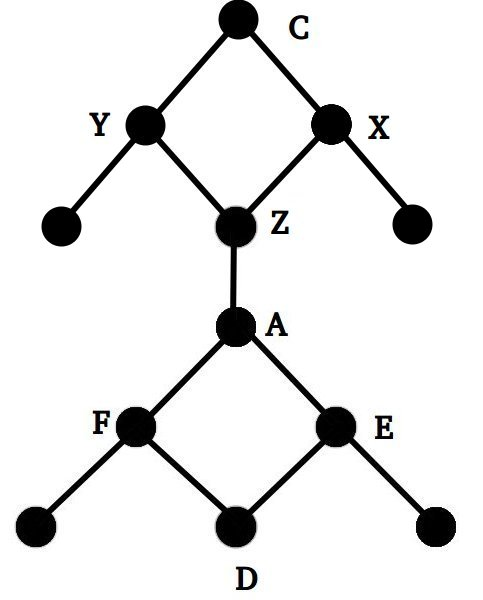
\includegraphics[scale=0.5]{example1.jpg}}
\caption{Four different paths between C and D, that share one edge.}
\label{ex1}
\end{figure}

Sometimes we prefer to remove GCIs that involve most specific concepts during contraction (this will be discussed in the coming chapter). To contract such GCIs, we can just remove, from each $C-D$ path, the edges going into $C$. In Figure \ref{ex1}, it would mean removing two edges: (C, X) and (C, Y). But removing such edges does not guarantee the minimum change. So we might end up having to choose which strategy is more preferred: minimal change or change with most specific concepts. The minimal hitting set approach that was mentioned earlier might not always satisfy specificity. So the user might have to choose which one to apply first, and which one to use as a tie breaker.

Removing the edges that involve nodes representing most specific concepts is straightforward; remove the edges that go into the most specific concept's node (C in our example). But it is not clear if one chooses to remove the least number of edges, instead, how this can be done. For this, we introduce an approach that uses the Minimum Cut algorithm to determine the minimum number of edges that need to be removed and identify them.

\subsubsection{Reduction to network flow problem}
As explained in \cite{alg}, the network flow problem is the problem of computing the maximum flow possible in a network (represented as a graph) by finding the minimum cut of the network. The input to the Ford-Fulkerson algorithm, that solves this problem, would be:
\begin{itemize}
\item A graph $G = (V, E)$.
\item A source $s \in V$.
\item A sink $t \in V$.
\item Capacity function $C:E \rightarrow \mathbb{N}$ representing the maximum capacity of each edge.
\end{itemize}

To contract $C \sqsubseteq D$ given the $TBox$ graph $G$, we choose $C$ to be the source, $D$ to be the sink, and we assume that the capacities of all edges are the same, equal to 1. The algorithm will find the maximum flow from $C$ to $D$, which is equal to the capacity of the minimum cut (the sum of capacities of the cut edges); we can then extract the edges that form that minimum cut and remove them.

The approach of removing the minimum cut edges of the graph is equivalent to the approach of removing the minimal hitting set formulas of the kernels. The minimal hitting set is the set containing the minimum number of elements that hit all sets, while the minimum cut of the graph is the minimum number of edges (since they all have the same capacity) that cover all paths from $C$ to $D$ (where edges represent GCIs of the $TBox$ and paths represent kernels.) So using the minimum cut approach should guarantee the minimum change for kernel contraction, as the minimal hitting set approach does.

Assuming we have a function ``Ford-Fulkerson(graph, s, t)'' that computes the maximum flow in the network (or graph) from source node ``s'' to a sink  ``t'' with edge-capacities ``1'', and returns the set of edges of the minimum cut, we can modify the contraction algorithm to adopt the minimum cut approach as in Algorithm \ref{GraphContract-modified}.

\begin{algorithm}
\caption{Another version of contraction algorithm}
\label{GraphContract-modified}
\begin{algorithmic}[1]
\Function {graphContractUsingMinCut}{$ \mathcal{T} $, $ \mathbb{A} $}
\State complete($ \mathcal{T} $)
\State graph = transform($ \mathcal{T} $)
\State C = $arg_{left}(\mathbb{A})$ $//arg_{left}$ gets the concept expression on the left side of the GCI
\State D = $arg_{right}(\mathbb{A})$ $//arg_{right}$ gets the right-side concept expression
\State min-cut = Ford-Fulkerson(graph, C, D)
\State remove min-cut edges from graph
\State $ \mathcal{T} $ = de-transform(graph)
\EndFunction
\end{algorithmic}
\end{algorithm}

For special cases such as contracting $C \sqsubseteq D1 \sqcap D2$, it is sufficient to contract $C \sqsubseteq D1$ first, and then contract $C \sqsubseteq D2$. But since the graph is already normalized (using complete() function), rules of the form $C \sqsubseteq D1 \sqcap D2$ are already broken down into two: $C \sqsubseteq D1$, and $C \sqsubseteq D2$. Therefore, the conjunction $\sqcap$ would only appear on the left hand side of a GCI in a normalized $TBox$ (e.g. $A1 \sqcap A2 \sqsubseteq B$). In that case, for contracting $A1 \sqcap A2 \sqsubseteq B$, there will be a node $A1 \sqcap A2$, which we will use as a source node; the sink would be the node representing $B$. 

As in \cite{alg}, the minimum cut algorithm runs in polynomial time. So using it in the contraction algorithm will not have a significant effect on the complexity of the main algorithm (will not elevate the complexity from being polynomial to being exponential). 

In some applications, the decision about which strategy to follow for choosing the edges to remove might vary depending on the situation. So the user can be asked in such case about which strategy to follow -- specificity or minimality. 

The last step of the algorithm is to transform the graph back to $\mathcal{EL}$. This can be done as follows: starting with an empty $TBox$ $\mathcal{T'}$, for every edge $(X, Y)$, add $X \sqsubseteq Y$ to $\mathcal{T'}$. The resulting $TBox$ would be the result of contracting $\mathcal{T}$ by $\mathbb{A}$. This is shown in Algorithm \ref{DeTransform}.

\begin{algorithm}
\caption{Transforming a graph back to a $TBox$}
\label{DeTransform}
\begin{algorithmic}[1]
\Function {de-transform}{graph}
\State result = $\{\}$
\State graph = (V, E)
\For{every $(X, Y) \in E$}
\State $result = result \cup \{X \sqsubseteq Y\}$
\EndFor
\State \Return result
\EndFunction
\end{algorithmic}
\end{algorithm}

Since the running time of every step of the contraction algorithm starting from ``transform($ \mathcal{T} $)'' until the last step is polynomial in the size of the $TBox$, the complexity of the algorithm will depend on the complexity of the first step (the complete() function). If building the subsumption hierarchy by generating all subsumptions of an $\mathcal{EL}$ $TBox$ can be done in polynomial time, then the contraction algorithm will in turn take polynomial time. But if generating all subsumptions takes exponential time, then the algorithm will take exponential running time as well.

\subsubsection{A Sample Run}
Suppose we have a TBox $\mathcal{T}$:
\begin{center}
$\mathcal{T} = \lbrace A \sqsubseteq B, B \sqsubseteq C \rbrace$
\end{center}
which implies $A \sqsubseteq C$. Trying to contract $\mathcal{T}$ by $A \sqsubseteq C$ using the network flow approach would work as follows:
\begin{enumerate}
\item complete($\mathcal{T}$). 
The TBox is already normalized. Translating it into a graph and applying the completion rules will introduce $A \sqsubseteq C$ and will be added explicitly to the TBox.
\item transform($\mathcal{T}$).
After transforming the TBox into a graph, it will look like the graph in Figure \ref{fig:abc-kb}.

\begin{figure}
\centering
\fbox{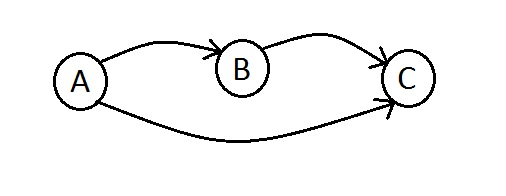
\includegraphics[scale=0.5]{abc-kb.jpg}}
\caption{Graph representing TBox $\mathcal{T} = \lbrace A \sqsubseteq B, B \sqsubseteq C, A \sqsubseteq C \rbrace $}
\label{fig:abc-kb}
\end{figure}

\item getPaths(graph, A, C) will get all paths between A and C. There are only two paths: A-B-C and A-C. 

\item Cutting the two paths A-B-C and A-C will be done by removing the edge between A and C, as well as one of the two edges A-B and B-C. So the resulting graph will only have one edge: A-B or B-C.

\item After transforming the graph again into a TBox, the result will be:
\begin{center}
$\mathcal{T} = \lbrace A \sqsubseteq B \rbrace$
\end{center}
or 
\begin{center}
$\mathcal{T} = \lbrace B \sqsubseteq C \rbrace$.
\end{center}

\end{enumerate}


\subsubsection{The limitations of the algorithm}
The previous example shows how the algorithm succeeds in finding the set of kernels by finding the paths from the source to the sink (where source and sink represent the two sides of the GCI that we need to remove). The example we will discuss now shows how the conjunction symbol ($\sqcap$) might introduces further complexity that the algorithm will not overcome. Given the TBox $\mathcal{T}$:
\begin{center}
$\mathcal{T} = \lbrace A \sqsubseteq B, A \sqsubseteq C, B \sqcap C \sqsubseteq D \rbrace$
\end{center}
we can see that it entails
\begin{center}
$A \sqsubseteq D$.
\end{center}
If we want to contract the TBox by $A \sqsubseteq D$, we would look for its kernels and remove a statement from each. In this example we have only one kernel:
\begin{center}
$\lbrace A \sqsubseteq B, A \sqsubseteq C, B \sqcap C \sqsubseteq D \rbrace$.
\end{center}
So removing one of the three GCIs is enough to give up $A \sqsubseteq D$. Contracting it using our graph approach works as follows:

\begin{enumerate}
\item complete($\mathcal{T}$). 
The TBox is already normalized. Translating it into a graph and applying the completion rules will introduce $A \sqsubseteq B \sqcap C$ and will be added explicitly to the TBox.
\item transform($\mathcal{T}$).
After transforming the TBox into a graph, it will look like the graph in Figure \ref{fig:abcbc-kb}.

\begin{figure}
\centering
\fbox{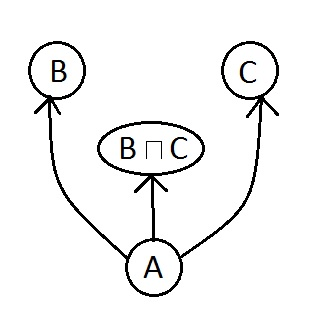
\includegraphics[scale=0.5]{abcbc-kb.jpg}}
\caption{Graph representing TBox $\mathcal{T} = \lbrace A \sqsubseteq B, A \sqsubseteq C, A \sqsubseteq B \sqcap C, B \sqcap C \sqsubseteq D \rbrace $}
\label{fig:abcbc-kb}
\end{figure}

\item getPaths(graph, $A$, $D$) will get all paths between $A$ and $D$. There is only one such path, which is $A -- B \sqcap C -- D$. So removing one of these two edges is the only possible outcomes of the algorithm.
\end{enumerate}

This last step is where the algorithm fails. It finds only one of the kernels because it does not recognize that the two parallel edges from $A$ to $B$ and $C$ actually form another kernel. This is because a kernel in our graph approach can only be represented as a path. The conjunction symbol $\sqcap$ has a different meaning, and is not analogous to the path notion. However, the algorithm worked with the previous example because the GCI we tried to remove was the result of applying the transitivity property of the subsumption symbol ($\sqsubseteq$) to two other GCIs and they together were represented by a path in the graph representation.

Similarly, we can argue that the algorithm also fails when the existential quantification symbol ($\exists$) is used. For example, the following TBox:
\begin{center}
$\mathcal{T} = \lbrace A \sqsubseteq \exists r.B, B \sqsubseteq C \rbrace$
\end{center}
implies the following expression:
\begin{center}
$A \sqsubseteq \exists r.C$
\end{center}
The graph approach will not get the kernels of that expression using the getPaths() function. So, it will also fail. But this is only because of the subsumption of $B$ by $C$, where $B$ is included in the role expression $\exists r.B$. If the existential quantification symbol is used without changing the symbols involved in the roles (such as $B$), the algorithm will work fine, as it will only be depending on the subsumption relations between concept expressions.

So it seems that the limitations of this algorithm are only due to the difference between the inference using paths between nodes and inference the introduces conjunction or existential quantification. However, the algorithm does not always fail when $\sqcap$ or $\exists$ is involved. In Figure \ref{fig:abc-kb}, if we replace B by (X $\sqcap$ Y), or by  ($\exists r.$B), the algorithm will succeed. That is because the nodes do not change after the inference; all that is added by the subsumption algorithm are new edges. 


\subsubsection{Analysis of the graph algorithm}
The analysis we refer to here is with respect to rationality. It is important to be able to measure the correctness of the solution we get from running the algorithm. Correctness could be measured by the rationality postulates that are expected to govern kernel contraction. We will examine each of the four postulates that Hansson mentioned in \cite{hansson} and see if the algorithm actually satisfies all of them.

\begin{description}
\item[Success] If $\alpha \notin Cn(\emptyset)$, then $\alpha \notin Cn(A \div \alpha)$.
\end{description}
Since according to the definitions of kernels, each kernel is one way to imply $\alpha$, and since we are incising all kernels (all paths), then the new set cannot not imply $\alpha$. So this postulate is satisfied.

\begin{description}
\item[Inclusion] $A \div \alpha \subseteq A$.
\end{description}
Since we are not adding any extra beliefs, and assuming $A$ is the normalized version of the TBox, then this postulate is also satisfied. It is safe to assume that $A$ is the normalized TBox because normalization does not change the belief set (or the epistemic state) of the agent, but it only changes the belief base by putting the beliefs in a form easier to contract.

\begin{description}
\item[Core-retainment] If $\beta \in A$ and $\beta \notin A \div \alpha$, then there is a set $A'$ such that $A' \subseteq A$ and that $\alpha \notin Cn(A')$ but $\alpha \in Cn(A' \cup \{ \beta \})$.
\end{description}
This postulate is also satisfied because we are only removing beliefs that contribute to the contracted belief, as the minimum cut actually represents the smallest set of sentences that can be removed to contract the knowledge by $\alpha$ (\textit{minimum change}).

\begin{description}
\item[Uniformity] If it holds for all subsets $A'$ of $A$ that $\alpha \in Cn(A')$ if and only if $\beta \in Cn(A')$, then $A \div \alpha = A \div \beta$.
\end{description}
Given the semantics of $\mathcal{EL}$, two GCIs can be equivalent if and only if they are exactly the same. So this requirement is trivially achieved.


\subsection{How to generate kernels?}
So far, we have discussed two ways for generating all kernels:
\begin{enumerate}
\item Using the pinpointing algorithm.
\item Using the graph approach.
\end{enumerate}
Computing kernels using the graph approach finds all kernels by performing depth-first search on the graph representation of the TBox. It finds all kernels in $O(E)$, where $E$ is the number of edges in the graph (or the number of GCIs in the TBox). However, it only works with subsumptions that do not include the conjunction symbol ($\sqcap$). So, in cases where the conjunction is not used in the TBox, the graph approach will be at least as efficient as the pinpointing approach, if not better (the axiom pinpointing algorithm introduced in \cite{pin} finds one kernel in polynomial time).


\subsection{What incision function to use?}
If we care about selecting minimum number of beliefs to remove, then there are two incision approaches we discussed so far:
\begin{enumerate}
\item The minimum hitting set algorithm.
\item The minimum cut algorithm for the network flow problem.
\end{enumerate}
The minimum hitting set problem is NP-hard. However, the algorithm we discussed in this study is a relatively efficient approximation algorithm. However, in cases where the minimum cut approach can be used, the minimum cut algorithm is probably the best and most efficient. The algorithm works by finding the max flow possible through the network build from the TBox, and then uses it to find the minimum cut.

The Ford-Fulkerson maximum flow algorithm typically takes $O(E \cdot F)$ steps to find the maximum flow, where $E$ is the number of edges and and $F$ is the value of the maximum flow. The value of $F$ is upper bounded by the the sum of all capacities, i.e. the maximum flow can never be greater than the sum of capacities of all edges. Since all edges in our approach has capacity 1, $F$ cannot exceed $E$. So the complexity of the algorithm can be reformulated as $O(E^2)$. After finding the maximum flow, we can find the minimum cut in $O(E)$. So the overall complexity of the algorithm is $O(E^2)$. Ford-Fulkerson algorithm is not polynomial-time, in general, because it depends on the value of the maximum flow, which is dependent on the capacities. There are other algorithms that are proved to be polynomial-time in general, such as the one introduced in \cite{preflow}. However, the application of Ford-Fulkerson algorithm here is always polynomial-time, because the capacities are all 1 which makes the maximum flow a polynomial function of the number of edges.

In other cases where the graph approach is not applicable, the minimum hitting set algorithm is a good candidate. In the next chapter, we will also give some techniques for implementing the incision function. Some of them might be even more suitable than the minimum hitting set approach, depending on the domain and the preferences of the user.